\section{Parallel FEM Poisson solver}
\begin{figure}[H]
    \centering
    \includegraphics[width=\textwidth]{figures/fempoisson_surface.png}
    \caption{Solution of the parallel FEM Poisson solver.}
    \label{fig:parallel_fem}
\end{figure}

\subsection{Data communication between neighbouring processes}
The data communication between neighbouring processes is implemented in the
\href{https://github.com/PhilipSoliman/hpc-labs/blob/96864119216b357345f2e0b75c3b423d411a9a99/assignment_2/MPI_Fempois.c#L517-L530}
{\lstinline[language=C]|Exchange_Borders()|}

\subsection{Benchmarking}
Figure \ref{fig:parallel_fem_benchmark} shows the timing results of the parallel FEM Poisson solver.
Note that I added one extra category for file I/O.

From the figure we see that the computation time is approximately the same for all processes for any grid size
and a given process topology. This is to be expected, as processes keep performing computations untill the global 
error criterion is met.

Additionally, assymetry in exchange is evident from the figure. I explain why this is so in 
section \ref{sec:communication_assymetry}. 

Lastly, we observe that a good portion of the root process' time is spent in file I/O. This is due 
to the fact that the root process is responsible for reading from the input and writing to final the solution to file. 
While it performs these tasks the other processes remain idle.

\begin{figure}[H]
    \centering
    \includegraphics[width=0.9\textwidth]{figures/fempoisson_benchmark.png}
    \caption{Benchmarking of the parallel FEM Poisson solver. Each bar corresponds
    to a process, rows correspond to grid sizes, columns correspond to the process topology
    and colours to thr different categeories of time; computation (blue),
    exchange/local communication (orange), global communication (green), 
    idle (red) and file I/O (purple).}
    \label{fig:parallel_fem_benchmark}
\end{figure}


\subsection{Data communication estimates}
Let $n$ and $p$ be the number of grid points and processes in each direction respectively. 
Any two neighbouring processes share $\frac{n}{p}$ vertices. Inner processes have 4 neighbours,
edge processes have 3 neighbours, and corner processes have 2 neighbours. There are $(p-2)^2$ inner
processes, $4(p-1)$ edge processes, and 4 corner processes. Hence the total number of shared vertices
is given by
\begin{align*}
    |V_{\textrm{shared}}| &= \frac{n}{p}\left(4(p-2)^2 + 12(p-1) + 8\right)\\
    &= \frac{n}{p}\left(4p^2 - 16p + 16 + 12p - 12 + 8\right)\\
    &= \frac{n}{p}\left(4p^2 - 4p + 12\right)\\
    &= \frac{4n}{p}\left(p^2 - p + 3\right),\\
\label{eq:shared_vertices}
\end{align*}
which holds for $p>3$ and $n\geq p$. Since a double is $8$ bytes and data is communicated in both 
directions, the total amount of communicated data per iteration is approximately given by
\begin{align*}
    B &= 16 |V_{\textrm{shared}}| [B]\\
    &= \frac{64n}{p}\left(p^2 - p + 3\right) [B].
\end{align*}

\subsection{Communication assymetry}
\label{sec:communication_assymetry}
From the function 
\href{https://github.com/PhilipSoliman/hpc-labs/blob/96864119216b357345f2e0b75c3b423d411a9a99/assignment_2/GridDist.c#L309-L322}
{\lstinline[language=C]|Write_Datafiles()|}
I deduce the communication pattern shown in Figure \ref{fig:parallel_fem_ambiguity},
which shows a sketch of the grid for $n=6$ and $p=3$. From this figure we see
that vertex exchange for the inner process $p_{11}$ takes place in 6 distinct locations and directions. 
This means that the inner process has 6 neighbours. In the figure we also see the communication of the 
corner process $p_{22}$ which only has 2 neighbours. 
\begin{figure}[H]
    \centering
    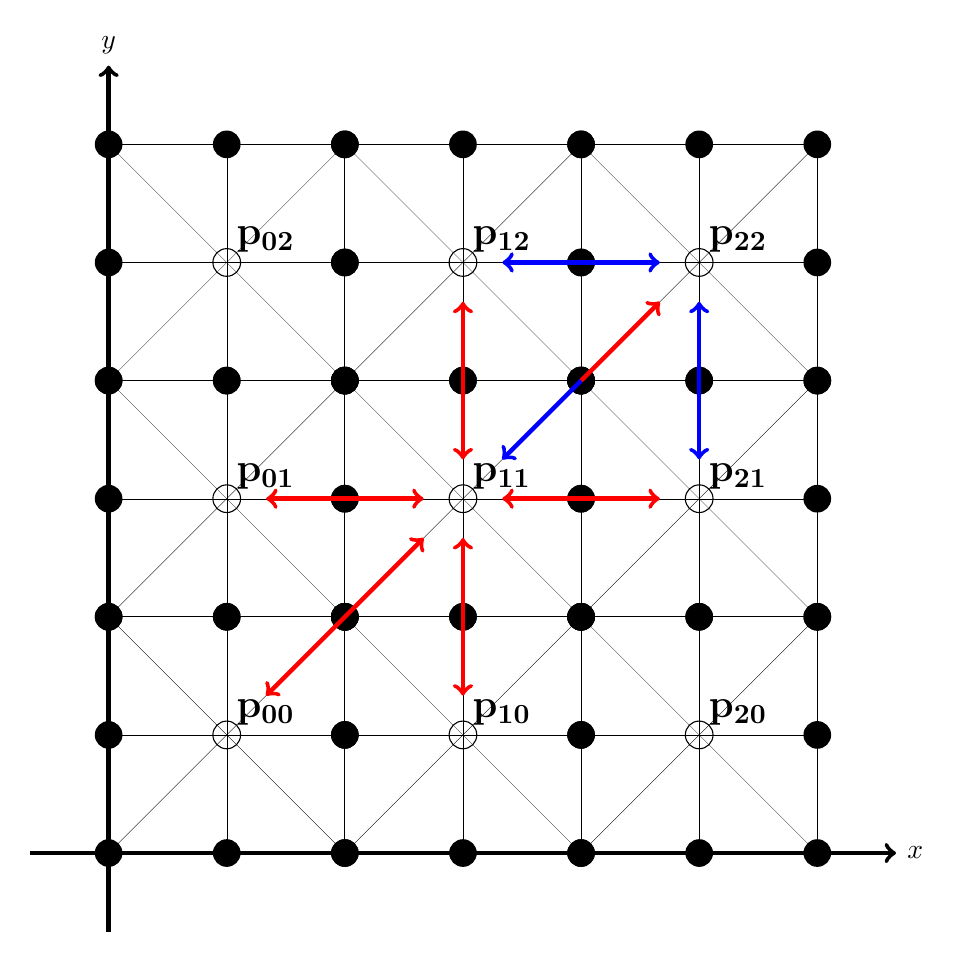
\begin{tikzpicture}

    % Draw the x and y axes
    \draw[->,ultra thick] (-1,0) -- (10,0) node[right] {$x$};
    \draw[->,ultra thick] (0,-1) -- (0,10) node[above] {$y$};

    % Draw process grid
    \foreach \i in {0,3,6,9} {
        \draw[thin] (\i,0) -- (\i,9);
        \draw[thin] (0,\i) -- (9,\i);
    }

    % Draw triangles and place dots on vertices
    \foreach \i in {0,3,6} {
        \foreach \j in {0,3,6} {
            % triangles
            \draw[ultra thin] (\i,\j) -- (\i+3,\j+3);
            \draw[ultra thin] (\i,\j+3) -- (\i+3,\j);
            \draw[ultra thin] (\i,\j+1.5) -- (\i+3,\j+1.5);
            \draw[ultra thin] (\i+1.5,\j) -- (\i+1.5,\j+3);

            % dots on vertices
            \fill[black] (\i,\j) circle (5pt);
            \fill[black] (\i+3,\j) circle (5pt);
            \fill[black] (\i,\j+3) circle (5pt);    
            \fill[black] (\i+3,\j+3) circle (5pt);
            \fill[black] (\i+1.5,\j) circle (5pt);
            \fill[black] (\i+1.5,\j+3) circle (5pt);
            \fill[black] (\i,\j+1.5) circle (5pt);
            \fill[black] (\i+3,\j+1.5) circle (5pt);
        }
    }

    % Add process labels
    \foreach \i in {0,1,2} {
        \foreach \j in {0,1,2} {
            \node at (3*\i+1.5,3*\j+1.5) [above right] {\Large $\mathbf{p_{\i\j}}$};
            \draw (3*\i+1.5,3*\j+1.5) circle (5pt);
        }
    }

    % Show neighbouring processes of p11
    \draw[->,red,ultra thick] (6,6) -- (7,7);
    \draw[<->,red,ultra thick] (2,2) -- (4,4);
    \draw[<->,red,ultra thick] (2,4.5) -- (4,4.5);
    \draw[<->,red,ultra thick] (5,4.5) -- (7,4.5);
    \draw[<->,red,ultra thick] (4.5,2) -- (4.5,4);
    \draw[<->,red,ultra thick] (4.5,5) -- (4.5,7);

    % Show neithering processes of p22
    \draw[<->,blue,ultra thick] (7.5,7) -- (7.5,5);
    \draw[<->,blue,ultra thick] (5,7.5) -- (7,7.5);
    \draw[<-,blue,ultra thick] (5,5) -- (6,6);



\end{tikzpicture}

    \caption{Sketch of gird for $n=6$ and $p=3$. Filled black circles represent shared vertices and 
    black circles represent the vertices of the internal vertices. In this example each process
    only contains one inner vertex. The red lines indicate vertex exchange between the inner process $p_11$ and its
    neighbours.}
    \label{fig:parallel_fem_ambiguity}
\end{figure}
Assymetry in communication stems from the fact that vertices located on the boundary 
of 4 processes are ambiguous w.r.t. which of those process they belong to. Hence 
we choose to exclusively link bottom-left and/or top-right neighbours. 

\subsection{Communication and computation overlap}
Figures \ref{fig:parallel_fem_overlap_gridsize} and \ref{fig:parallel_fem_overlap_processors} show the
communication and computation overlap in the parallel FEM Poisson solver defined as
\begin{equation}
    \textrm{overlap} = \frac{\textrm{computation time}}{\textrm{communication time}}.
\end{equation}
\begin{figure}[H]
    \centering
    \includegraphics[width=0.9\textwidth]{figures/fempoisson_overlap_vs_gridsize.png}
    \caption{
        Communication (global + local) and computation overlap in the parallel FEM Poisson solver for $2\times2$ 
        and $4\times1$ processes plotted against gridsize.}
    \label{fig:parallel_fem_overlap_gridsize}
\end{figure}
\begin{figure}[H]
    \centering
    \includegraphics[width=0.9\textwidth]{figures/fempoisson_overlap_vs_processes.png}
    \caption{
        Communication (global + local) and computation overlap in the parallel FEM Poisson solver plotted against
        number of processes.}
    \label{fig:parallel_fem_overlap_processors}
\end{figure}
From the above figures we see that for fixed $p=4$ and a regular grid, the communication and computation overlap equals 1 for 
grid sizes $g=35\ \textrm{to}\ 40$ depending on process topology. This means that the computation time is approximately equal to the
communication time. For the adaptive grid, the overlap is approximately 1 for $g=50$.

Similarly, for a fixed $g=100$ and a regular grid, the overlap (approximately) equals 1 for $p=6$ and is 
predicted to be below 1 for $p>7$. The experiment is inconclusive for the adaptive grid, but the overlap is 
close to onr for $p=4$ and 5.

\subsection{Adaptive grid refinement}
Figure \ref{fig:parallel_fem_adaptive_refinement} shows the Effect of adaptive grid refinement on error evolution 
\begin{figure}[H]
    \centering
    \includegraphics[width=0.7\textwidth]{figures/fempoisson_error_evolution.png}
    \caption{Error evolution for $g=100,200,400$ for both process topologies and on (non-)adaptive grids.
    Rows correspond to grid sizes, columns correspond to the process topology, blue lines
    to non-adaptive grids and orange lines to adaptive grids. On the top right of each plot 
    the relative percentual speedup is shown, where negative values indicate a faster computation time
    for the adaptive grid.}
    \label{fig:parallel_fem_adaptive_refinement}
\end{figure}


